\documentclass{beamer}
%\documentclass[handout]{beamer}

\usepackage[ngerman]{babel}
\usepackage[latin1]{inputenc}
\usepackage[T1]{fontenc}
\usepackage{lmodern}
\usepackage{tikz}
\usepackage{pgfplots}

% VSIS-Theme verwenden
\usetheme{vsis}

% Vor jedem neuen Teil (\part) eine Folie mit Titel anzeigen
\AtBeginPart{\frame{\partpage}}

% Vor jedem neuen Abschnitt (\section) eine Folie mit Gliederung f�r diesen Abschnitt zeigen
\AtBeginSection{\frame{\frametitle{\insertsection}\tableofcontents[currentsection,hideothersubsections]}}

% f�r Grafik-Beispiel:
\usepackage{tikz}
\usetikzlibrary{arrows,positioning,fit,backgrounds,shapes}

% Daten dieser Pr�sentation
\title{Cleaning von Zeitreihen}
\subtitle{Von der Anomalienerkennung zur Anomalienreparatur}
\author[Jose, Klaus]{Jose Rodriguez Parra Flores \\ Klaus-Johan Ziegert}
%\date{9.\ April 2009}
%\institute[Uni-HH]{Universit�t Hamburg \\ Fakult�t f�r Mathematik, Informatik und Naturwissenschaften \\ Department Informatik \\ Zentrum f�r Verteilte Informations- und Kommunikationssysteme \\ Arbeitsbereich Verteilte Systeme und Informationssysteme}

\definecolor{ao}{rgb}{0.0, 0.5, 0.0}

\newcommand{\smiley}{\tikz[baseline=-0.75ex,black]{
    \color{ao}
    \draw circle (2mm);
\node[fill,circle,inner sep=0.5pt] (left eye) at (135:0.8mm) {};
\node[fill,circle,inner sep=0.5pt] (right eye) at (45:0.8mm) {};
\draw (-145:0.9mm) arc (-120:-60:1.5mm);
    }
}

\newcommand{\frownie}{\tikz[baseline=-0.75ex,black]{
    \color{red}
    \draw circle (2mm);
\node[fill,circle,inner sep=0.5pt] (left eye) at (135:0.8mm) {};
\node[fill,circle,inner sep=0.5pt] (right eye) at (45:0.8mm) {};
\draw (-145:0.9mm) arc (120:60:1.5mm);
    }
}

\newcommand{\neutranie}{\tikz[baseline=-0.75ex,black]{
    \color{black}
    \draw circle (2mm);
\node[fill,circle,inner sep=0.5pt] (left eye) at (135:0.8mm) {};
\node[fill,circle,inner sep=0.5pt] (right eye) at (45:0.8mm) {};
\draw (-135:0.9mm) -- (-45:0.9mm);
    }
}


\begin{document}

\maketitle

\begin{frame}{Gliederung}
  \tableofcontents[hideallsubsections]
\end{frame}


\section{Einf�hrung}

\subsection{Motivation}

\begin{frame}{\insertsubsection}
  \begin{block}<+->{Messger�te liefern unzuverl�ssige Daten}
    \begin{itemize}
      \item GPS Tracker sind nahe von Geb�uden unzuverl�ssig
      \item Sensoren sind empfindlich gegen�ber �u�ere Einfl�sse
          \begin{itemize}
              \item Z.B. starker Fall der Temperaturen bei einem Windzug
          \end{itemize}
    \end{itemize}
  \end{block}
\begin{figure}
    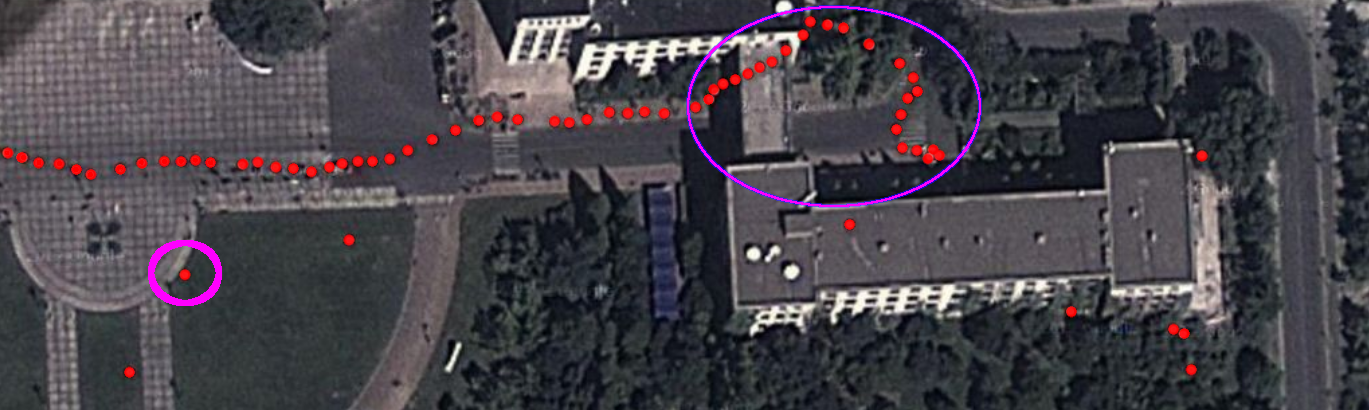
\includegraphics[width=\textwidth]{GPS_Motivation_Example.png}
    \caption{GPS-Tracking auf dem Campus der Tsinghua Universit�t \cite{Shaoxu17}}

\end{figure}

\end{frame}

\begin{frame}{\insertsubsection}
  \begin{block}<+->{Umgang von unzuverl�ssigen Daten mit Anomalienerkennung}
    \begin{enumerate}
        \item Unzuverl�ssige Datenpunkte entfernen
            \begin{itemize}
                \item Ausrei�er werden entfernt  \smiley
                \item Entfernen aufeinanderfolgende Fehler machen Ergebnis unbrauchbar \textbf{oder}
                 werden als solche ggf. nicht erkannt \frownie
            \end{itemize}
        \item Unzuverl�ssige Datenpunkte reparieren
            \begin{itemize}
                \item Einzelne Ausrei�er werden leicht korrigiert \neutranie
                \item Aufeinanderfolgende Fehler werden zu stark ver�ndert (In der Praxis liegen die Messungen nahe bei den korrekten Werten) \neutranie
            \end{itemize}
    \end{enumerate}
  \end{block}
\end{frame}

\begin{frame}{\insertsubsection}
    \begin{block}<+->{Hinzunahme von als wahr markierte Werte}
    \begin{enumerate}
        \item Markierung durch den Benutzer
            \begin{itemize}
            \item Z.B. markiert der Benutzer in beliebigen Zeitabst�nden seinen aktuellen Standort
            \end{itemize}
        \item Pr�zise Messger�te liefern in l�ngeren Zeitabst�nde korrekte Werte
    \end{enumerate}
  \end{block}
    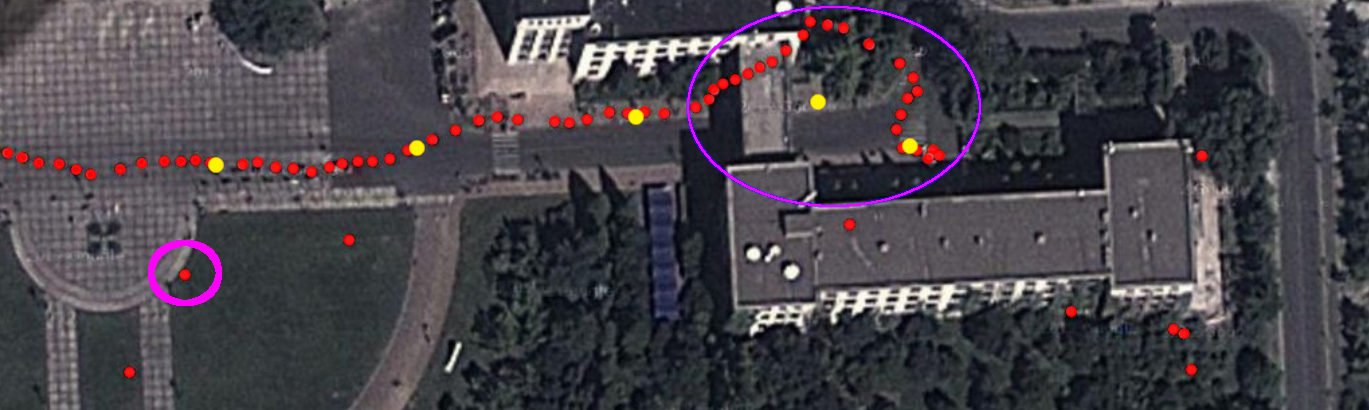
\includegraphics[width=\textwidth]{markierte_GPS_Motivation_Example.png}
\end{frame}



\subsection{Zielsetzung}

\begin{frame}{\insertsubsection}
  \begin{block}<+->{Ziel der Arbeit}
    \begin{enumerate}
      \item Einfliessen der markierten Werte in die Anomalienerkennung
            \begin{itemize}
                \item Aufeinanderfolgende Fehler sollen besser abgesch�tzt werden
            \end{itemize}
      \item Anomalienreparatur mit den Minimum-Change-Prinzip vereinbaren   
            \begin{itemize}
                \item Keine drastische Ver�nderungen der Messwerte
            \end{itemize}
      \item Einfliessen der markierten Werte in die anderen State-of-Art Verfahren
      \item Neue Anomalienreparatur mit den anderen Verfahren empirisch vergleichen
    \end{enumerate}
  \end{block}
\end{frame}



\section{Grundlagen}

\subsection{Problemstellung}

\begin{frame}{\insertsubsection}
  \begin{block}<+->{Zeitreihenreparatur}
    \begin{itemize}
        \item Gegeben:
            \begin{itemize}
                \item Eine fehlerbehafte Messung $x = x[1],\dots,x[n]$
                \item Eine unvollst�ndige, aber daf�r ausschlie�lich korrekte Messung $x^{\text{truth}}$
            \end{itemize}
        \item Gesucht:
            \begin{itemize}
                \item Reparatur $y$ mit minimalen RMS-Fehler $\Delta(x^{\text{truth*}}, y)$
                \item $\Delta(x^{\text{truth*}}, y) = \sqrt{\frac{1}{n} \sum_{i=1}^{n} \left(x_i^{\text{truth*}} - y_i\right)^2 }$
            \end{itemize}
    \end{itemize}
  \end{block}
\end{frame}

\subsection{Anomalienreparaturen}

\begin{frame}{\insertsubsection}
  \begin{block}<+->{Blank}
    \begin{itemize}
      \item Fakten
      \item Fakten
      \item Fakten \cite{zhang17}
    \end{itemize}
  \end{block}
\end{frame}

\subsection{andere Verfahren}

\begin{frame}{\insertsubsection}
  \begin{block}<+->{Blank}
    \begin{itemize}
      \item Fakten
      \item Fakten
      \item Fakten
    \end{itemize}
  \end{block}
\end{frame}

\section{Iterative Minimum Repairing}

\subsection{IMR}

\begin{frame}{\insertsubsection\ Intuition}
    \begin{block}{Intuitiver Ansatz von IMR}
        \begin{itemize}
            \item ARX nutzt markierte Werte effizient, \textbf{aber} ver�ndert die Werte zu drastisch.
            \item IMR Ansatz:
                \begin{enumerate}
                    \item Wende ARX an
                    \item W�hle \textbf{einen} Reparaturwert mit minimalen Abstand zur Messung
                    \item Wiederhole Prozedur bis aktuelle Reparatur sich nicht signifkant �ndert
                \end{enumerate}
            \item Motivation: Reparierte Werte verbessern zuk�nftige Reparaturen 
        \end{itemize}
    \end{block}
\end{frame}

\begin{frame}[fragile]{\insertsubsection\ = ARX + Minimum-Change-Prinzip}
    \begin{algorithm}[H]
    \begin{algorithmic}[1]
\STATE \textbf{Eingabe}: Messung $x$, markierte Werte $x^{\text{truth}}$, Ordnung $p$, Schwellenwert $\tau$ und max-num-iterations
\STATE \textbf{Ausgabe}: Reparatur $y$ 
        \STATE {$y^{(0)} \gets$ Initialize$(x,x^{\text{truth}})$}
\FOR{$k \gets 0$ \TO max-num-iterations}
\STATE {$\phi^{(k)} \gets$ Estimate$(x,y^{(k)})$}
    \STATE { $\hat{y} \gets$ Candidate$(x,y^{(k)}, \phi^{(k)})$}
    \STATE { $y^{(k+1)} \gets$ Evaluate$(x,y^{(k)}, \hat{y})$}
        \IF{ Converge($y^{(k)}, y^{(k+1)}$) }
        \STATE {\textbf{break}}
        \ENDIF
 \ENDFOR
    \RETURN $y^{(k)}$
\end{algorithmic}
\end{algorithm}
\end{frame}

\begin{frame}[fragile]{\insertsubsection:\ Initialisierung}
    \begin{algorithm}[H]
    \begin{algorithmic}[1]
\STATE \textbf{Eingabe}: Messung $x$, markierte Werte $x^{\text{truth}}$, Ordnung $p$, Schwellenwert $\tau$ und max-num-iterations
\STATE \textbf{Ausgabe}: Reparatur $y$ 
        \STATE \colorbox{blue!30}{{$y^{(0)} \gets$ Initialize$(x,x^{\text{truth}})$}}
\FOR{$k \gets 0$ \TO max-num-iterations}
\STATE {$\phi^{(k)} \gets$ Estimate$(x,y^{(k)})$}
    \STATE { $\hat{y} \gets$ Candidate$(x,y^{(k)}, \phi^{(k)})$}
    \STATE { $y^{(k+1)} \gets$ Evaluate$(x,y^{(k)}, \hat{y})$}
        \IF{ Converge($y^{(k)}, y^{(k+1)}$) }
        \STATE {\textbf{break}}
        \ENDIF
 \ENDFOR
    \RETURN $y^{(k)}$
\end{algorithmic}
\end{algorithm}
\end{frame}

\begin{frame}[fragile]{\insertsubsection:\ Initialisierung}
    \begin{block}{Initiale Reparatur}
        Initiale Reparatur $y^{(0)}$ ist Messung $x$ und �bernimmt die markierten Werte aus $x^{\text{truth}}$
    \end{block}
    \begin{tikzpicture}
\begin{axis}[width=.8\textwidth,
   height=.4\textwidth,
xlabel=Zeitpunkt,
ylabel=Datenpunkt,
legend pos=outer north east,
xmin=0,
xmax=12,
ymin=5
]
\addplot[black, line width=2.0pt, mark size=2.0pt, mark=*]  table{
zeitpunkt wert 
1 6
2 10
3 9.6
4 8.3
5 7.7
6 5.4
7 5.6
8 5.9
9 6.3
10 6.8
11 7.5
12 8.5
};
\addlegendentry{$x$}
\addplot[only marks, red, mark size=5.0pt] table{
zeitpunkt wert 
1 6
2 5.6
3 5.4
6 5.4
12 8.5
};
\addlegendentry{$x^{\text{truth}}$}
    \addplot[olive,mark size=5.0pt, mark=x, line width=1.5pt] table{
    zeitpunkt wert 
    1 6
    2 5.6
    3 5.4
4 8.3
5 7.7
    6 5.4
    7 5.6
    8 5.9
    9 6.3
    10 6.8
    11 7.5
    12 8.5
    };
    \addlegendentry{$y^{0}$}
\end{axis}
\end{tikzpicture}

\end{frame}

\begin{frame}[fragile]{\insertsubsection: ARX auf aktuelle Reparatur anwenden}
    \begin{algorithm}[H]
    \begin{algorithmic}[1]
\STATE \textbf{Eingabe}: Messung $x$, markierte Werte $x^{\text{truth}}$, Ordnung $p$, Schwellenwert $\tau$ und max-num-iterations
\STATE \textbf{Ausgabe}: Reparatur $y$ 
        \STATE {$y^{(0)} \gets$ Initialize$(x,x^{\text{truth}})$}
\FOR{$k \gets 0$ \TO max-num-iterations}
        \STATE \colorbox{blue!30}{{$\phi^{(k)} \gets$ Estimate$(x,y^{(k)})$}}
        \STATE \colorbox{blue!30}{{ $\hat{y} \gets$ Candidate$(x,y^{(k)}, \phi^{(k)})$}}
    \STATE { $y^{(k+1)} \gets$ Evaluate$(x,y^{(k)}, \hat{y})$}
        \IF{ Converge($y^{(k)}, y^{(k+1)}$) }
        \STATE {\textbf{break}}
        \ENDIF
 \ENDFOR
    \RETURN $y^{(k)}$
\end{algorithmic}
\end{algorithm}
\end{frame}

\begin{frame}[fragile]{\insertsubsection:\ ARX auf aktuelle Reparatur anwenden}
    \begin{block}{Kandidaten}
        \begin{itemize}
            \item Parametersch�tzung $\phi$: aktuelle Reparatur $y^{(k)}$ wird als $x^{\text{truth}}$ interpretiert.
            \item Kandidaten $\hat{y}$ sind neue Reparaturwerte
        \end{itemize}
    \end{block}
\begin{tikzpicture}
\begin{axis}[width=.8\textwidth,
   height=.40\textwidth,
xlabel=Zeitpunkt,
ylabel=Datenpunkt,
legend pos=outer north east,
xmin=0,
xmax=12,
ymin=5
]
\addplot[black, line width=2.0pt, mark size=2.0pt, mark=*]  table{
Zeitpunkt Wert 
1 6
2 10
3 9.6
4 8.3
5 7.7
6 5.4
7 5.6
8 5.9
9 6.3
10 6.8
11 7.5
12 8.5
};
\addlegendentry{$x$}
\addplot[only marks, red, mark size=5.0pt] table{
Zeitpunkt Wert 
1 6
2 5.6
3 5.4
6 5.4
12 8.5
};
\addlegendentry{$x^{\text{truth}}$}
\addplot[only marks, olive,mark size=5.0pt] table{
Zeitpunkt Wert 
4 6.2
5 7.7
7 5.6
8 5.9
9 6.3
10 6.8
11 7.5
};
   \addlegendentry{$\hat{y}$}
% if you have the file, you can do
% \addplot table {datafile.csv};
\end{axis}
\end{tikzpicture}

\end{frame}

\begin{frame}[fragile]{\insertsubsection: Minimum-Change}
    \begin{algorithm}[H]
    \begin{algorithmic}[1]
\STATE \textbf{Eingabe}: Messung $x$, markierte Werte $x^{\text{truth}}$, Ordnung $p$, Schwellenwert $\tau$ und max-num-iterations
\STATE \textbf{Ausgabe}: Reparatur $y$ 
        \STATE {$y^{(0)} \gets$ Initialize$(x,x^{\text{truth}})$}
\FOR{$k \gets 0$ \TO max-num-iterations}
\STATE {$\phi^{(k)} \gets$ Estimate$(x,y^{(k)})$}
    \STATE { $\hat{y} \gets$ Candidate$(x,y^{(k)}, \phi^{(k)})$}
        \STATE { \colorbox{blue!30}{$y^{(k+1)} \gets$ Evaluate$(x,y^{(k)}, \hat{y})$}}
        \IF{ Converge($y^{(k)}, y^{(k+1)}$) }
        \STATE {\textbf{break}}
        \ENDIF
 \ENDFOR
    \RETURN $y^{(k)}$
\end{algorithmic}
\end{algorithm}
\end{frame}

\begin{frame}[fragile]{\insertsubsection:\ Minimum-Change}
    \begin{block}{Minimum-Change}
        \begin{itemize}
            \item Zu geringe �nderungen werden herausgefiltert $|y^{(k)}_i - \hat{y}_i| > \tau$
            \item Geringste �nderung zu Messung $x$ wird als Kandidat ausgew�hlt
        \end{itemize}
    \end{block}
\begin{tikzpicture}
\begin{axis}[width=.8\textwidth,
   height=.40\textwidth,
xlabel=Zeitpunkt,
ylabel=Datenpunkt,
legend pos=outer north east,
xmin=0,
xmax=12,
ymin=5
]
\addplot[black, line width=2.0pt, mark size=2.0pt, mark=*]  table{
Zeitpunkt Wert 
1 6
2 10
3 9.6
4 8.3
5 7.7
6 5.4
7 5.6
8 5.9
9 6.3
10 6.8
11 7.5
12 8.5
};
\addlegendentry{$x$}
\addplot[only marks, red, mark size=5.0pt] table{
Zeitpunkt Wert 
1 6
2 5.6
3 5.4
6 5.4
12 8.5
};
\addlegendentry{$x^{\text{truth}}$}
\addplot[olive,mark size=5.0pt, mark=x, line width=1.5pt] table{
Zeitpunkt Wert 
    1 6
    2 5.6
    3 5.4
4 6.2
5 7.7
    6 5.4
7 5.6
8 5.9
9 6.3
10 6.8
11 7.5
12 8.5
};
    \addlegendentry{$y^{(1)}$}
% if you have the file, you can do
% \addplot table {datafile.csv};
\end{axis}
\end{tikzpicture}

\end{frame}

\begin{frame}[fragile]{\insertsubsection: Terminierung}
    \begin{algorithm}[H]
    \begin{algorithmic}[1]
\STATE \textbf{Eingabe}: Messung $x$, markierte Werte $x^{\text{truth}}$, Ordnung $p$, Schwellenwert $\tau$ und max-num-iterations
\STATE \textbf{Ausgabe}: Reparatur $y$ 
        \STATE {$y^{(0)} \gets$ Initialize$(x,x^{\text{truth}})$}
        \FOR{\colorbox{blue!30}{$k \gets 0$ \TO max-num-iterations}}
\STATE {$\phi^{(k)} \gets$ Estimate$(x,y^{(k)})$}
    \STATE { $\hat{y} \gets$ Candidate$(x,y^{(k)}, \phi^{(k)})$}
    \STATE { $y^{(k+1)} \gets$ Evaluate$(x,y^{(k)}, \hat{y})$}
        \IF{\colorbox{blue!30}{Converge($y^{(k)}, y^{(k+1)}$) }}
        \STATE {\colorbox{blue!30}{\textbf{break}}}
        \ENDIF
 \ENDFOR
    \RETURN $y^{(k)}$
\end{algorithmic}
\end{algorithm}
\end{frame}

\begin{frame}{\insertsubsection: Terminierung}
    \begin{block}{Terminierung}
        \begin{itemize}
            \item Zwei M�glichkeiten der Terminierung:
        \begin{itemize}
            \item Maximale Anzahl der Iterationen wird erreicht
            \item Konvergenz: Neue Reparatur $y^{(k+1)}$ ist gleich aktuelle Reparatur $y^{(k)}$
        \end{itemize}
    \item Allgemeine Konvergenzfrage ist noch offen
        \end{itemize}
    \end{block}

\end{frame}

\subsection{Optimierung 1: Matrix-Pruning IMR}
\begin{frame}{Motivation von Matrix-Pruning IMR}
    \begin{block}{Laufzeit- \& Platzproblem}
        \begin{itemize}
            \item Parametersch�tzung beansprucht viel Zeit und Platz
            \item Matrizen V und Z bestehen aus $y_i^{(k)} - x_i$:
                \begin{itemize}
                    \item wenige markierte Werte vorhanden
                    \item markierte Werte h�ufig identisch zur Messung
                    \item Reparaturwerte �ndern sich nicht signifkant
                    \item $\rightarrow$ d�nnbesetzte Matrizen
                \end{itemize}
            \item Matrix-Pruning: L�schen von Zeilen mit 0en
        \end{itemize}
    \end{block}
\end{frame}

\begin{frame}{Matrix Pruning IMR Beispiel}
    \begin{block}{Beispiel}
        Zeilen mit 0en in Z und entsprechende Zeile in V sind entfernbar:
        \[
            Z =
            \left(
\begin{array}{c}
0\\
-4.4\\
-4.2\\
0\\
0\\
0\\
0\\
0\\
0\\
0\\
0\\
\end{array}
\right)
            V =
            \left(
\begin{array}{c}
-4.4\\
-4.2\\
0\\
0\\
0\\
0\\
0\\
0\\
0\\
0\\
0\\
\end{array}
\right)
\rightarrow
            Z_{mp} =
            \left(
\begin{array}{c}
-4.4\\
-4.2\\
\end{array}
\right)
            V_{mp} =
            \left(
\begin{array}{c}
-4.2\\
0\\
\end{array}
        \right)
        \]
    \end{block}
\end{frame}


\section{Evaluierung}

\subsection{Ordnung}

\begin{frame}{\insertsubsection}
  \begin{block}<+->{Blank}
    \begin{itemize}
      \item Fakten
      \item Fakten
      \item Fakten
    \end{itemize}
  \end{block}
\end{frame}

\subsection{Schwellenwert}

\begin{frame}{\insertsubsection}
  \begin{block}<+->{Blank}
    \begin{itemize}
      \item Fakten
      \item Fakten
      \item Fakten
    \end{itemize}
  \end{block}
\end{frame}

\subsection{maximale Anzahl von Iterationen}

\begin{frame}{\insertsubsection}
  \begin{block}<+->{Blank}
    \begin{itemize}
      \item Fakten
      \item Fakten
      \item Fakten
    \end{itemize}
  \end{block}
\end{frame}

\subsection{Markierungsrate}

\begin{frame}{\insertsubsection}
  \begin{block}<+->{Blank}
    \begin{itemize}
      \item Fakten
      \item Fakten
      \item Fakten
    \end{itemize}
  \end{block}
\end{frame}

\section{Schluss}

\subsection{Zusammenfassung und Ausblick}

\begin{frame}{\insertsubsection}
  \begin{block}<+->{Zusammenfassung}
    \begin{itemize}
      \item Was wurde getan?
    \end{itemize}
  \end{block}
  \begin{block}<+->{Ausblick}
    \begin{itemize}
      \item Wie k�nnten zuk�nftige Arbeiten aussehen?
    \end{itemize}
  \end{block}
\end{frame}



\subsection{Literatur}

\begin{frame}[allowframebreaks]{\insertsubsection}
  \begingroup
  \small
  \beamertemplatebookbibitems
  \bibliographystyle{plain}
  \bibliography{Beispiel}
  \endgroup
\end{frame}





\end{document}
